\chapter{Evaluation}


To ensure that the prototype satisfied our final problem statement, we had to evaluate our prototype through an usability and user experience combined test. 

\section{The usability test}
In order to find out to which degree out prototype met our usability and user experience requirements, we conducted a combined usability and user experience test

\subsection{Test goals}
The main goal of this test was to figure out if our target group perceived the prototype's usability and that the user experience was satisfaction. Although our original idea was that this test should be tested on our experts, unfortunately this was not possible which led us to test the prototype on regular students from AAU CPH, but in role as a garden designer and the customer.
Efficiency??
Learnability??
Safety???

\subsection{Sampling}
The combined usability test was conducted with the help of (number) participants. We used convenience sampling to find students at AAU CPH.

\subsection{Test specifics}

\subsection*{The equipment being used during the test}

\subsection*{Location and schedule}

\subsection*{Test procedure}

\subsection{Result}

\subsection{Findings}


\begin{figure}[H]
	\centering
	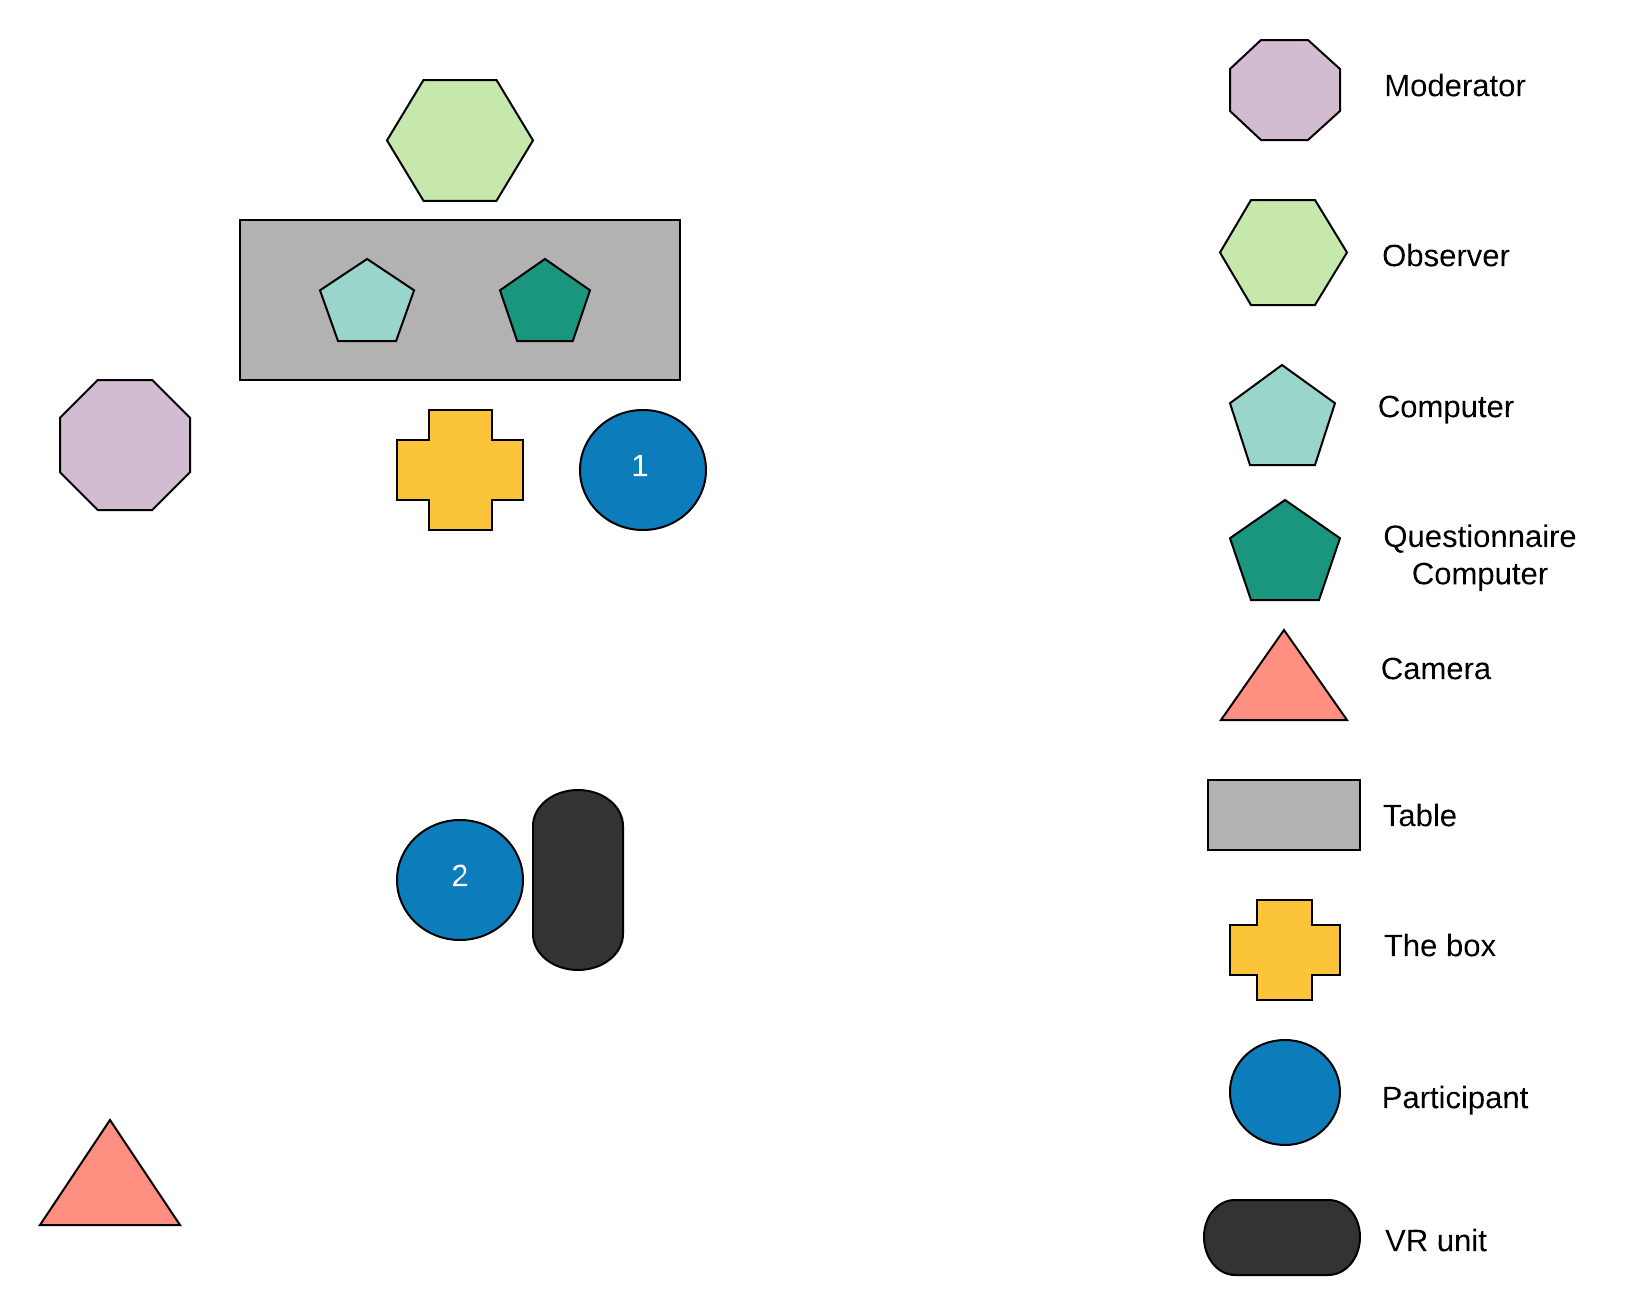
\includegraphics[width=1\linewidth]{figure/Evaluation/Test1.png}
	\caption{Our test setup, with the location of the participant, moderator, video camera and equipment. The two phases are visualized by the numbers in the circles.}
	\label{fig:test1}
\end{figure}